\documentclass[conference]{IEEEtran}
\IEEEoverridecommandlockouts
\usepackage{cite}
\usepackage{amsmath,amssymb,amsfonts}
\usepackage{algorithmic}
\usepackage{graphicx}
\usepackage{textcomp}
\usepackage{xcolor}
\usepackage{gensymb}
\usepackage{siunitx}
\usepackage{booktabs}
\usepackage{flushend}

\graphicspath{{robot_python_code/}}

\begin{document}

\title{Autonomous Navigation with EDT Path Planning and MPPI Control}

\author{
\IEEEauthorblockN{Karthik Shivashankaran}
\IEEEauthorblockA{
New York University Tandon School of Engineering\\
Brooklyn, NY, USA
}
}

\maketitle

\begin{abstract}
This report presents the design, implementation, and evaluation of a complete autonomous navigation pipeline for a four-wheeled mobile robot. The system represents the environment as an Euclidean Distance Transform (EDT) occupancy grid, uses Dijkstra's algorithm to compute a wall-clearance-aware global reference path, and applies Model Predictive Path Integral (MPPI) control to track that path while avoiding obstacles. A Monte Carlo Particle Filter (PF) with $N{=}1{,}000$ particles provides real-time pose estimates from RPLidar scans. The vectorized MPPI implementation samples $K{=}100$ trajectories over a horizon of $T{=}60$ steps and completes each iteration in 1.5--2.5\,ms, well within the 100\,ms control cycle. The PF converges from an unknown starting position within approximately 1\,s of motion, and the full pipeline loop runs in 40--42\,ms.
\end{abstract}

\section{Introduction}
Autonomous mobile robot navigation requires a representation of the environment, a mechanism for pose estimation, global path planning, and local collision-free control. This work integrates all four into a single pipeline running at 10\,Hz on a laptop communicating wirelessly with an Ackermann-steered robot.

The environment is modelled as a pre-surveyed wall polygon rasterized into an EDT grid that stores per-cell clearance to the nearest obstacle. Dijkstra's algorithm runs on a clearance-weighted graph derived from that grid to produce a globally optimal reference path whenever the operator specifies a goal. Pose estimation is performed by a Monte Carlo Particle Filter (PF) whose weighted mean drives the MPPI planner. MPPI selects steering commands by sampling trajectory perturbations and weighting them through a composite cost that combines wall proximity (via the EDT), path deviation, heading alignment, and goal distance.

Section~\ref{sec:method} details the mathematical formulation of each module. Section~\ref{sec:design} describes the hardware and experimental procedure. Section~\ref{sec:results} presents quantitative timing and localization results. Section~\ref{sec:conclusion} summarizes findings and future directions.

\section{Method}
\label{sec:method}

\subsection{System Overview}
The robot state is the planar pose $\mathbf{x}_t = [x_t,\, y_t,\, \theta_t]^\top$. At each 100\,ms tick the control loop executes four sequential steps:
\begin{enumerate}
    \item Receive the latest encoder count and steering angle via UDP.
    \item Update the PF with odometry and current LiDAR scan.
    \item Run one MPPI iteration using the PF mean as the current state estimate.
    \item Transmit the selected speed and steering command to the Arduino.
\end{enumerate}
Figure~\ref{fig:robot} shows the physical platform.

\begin{figure}[htbp]
\centerline{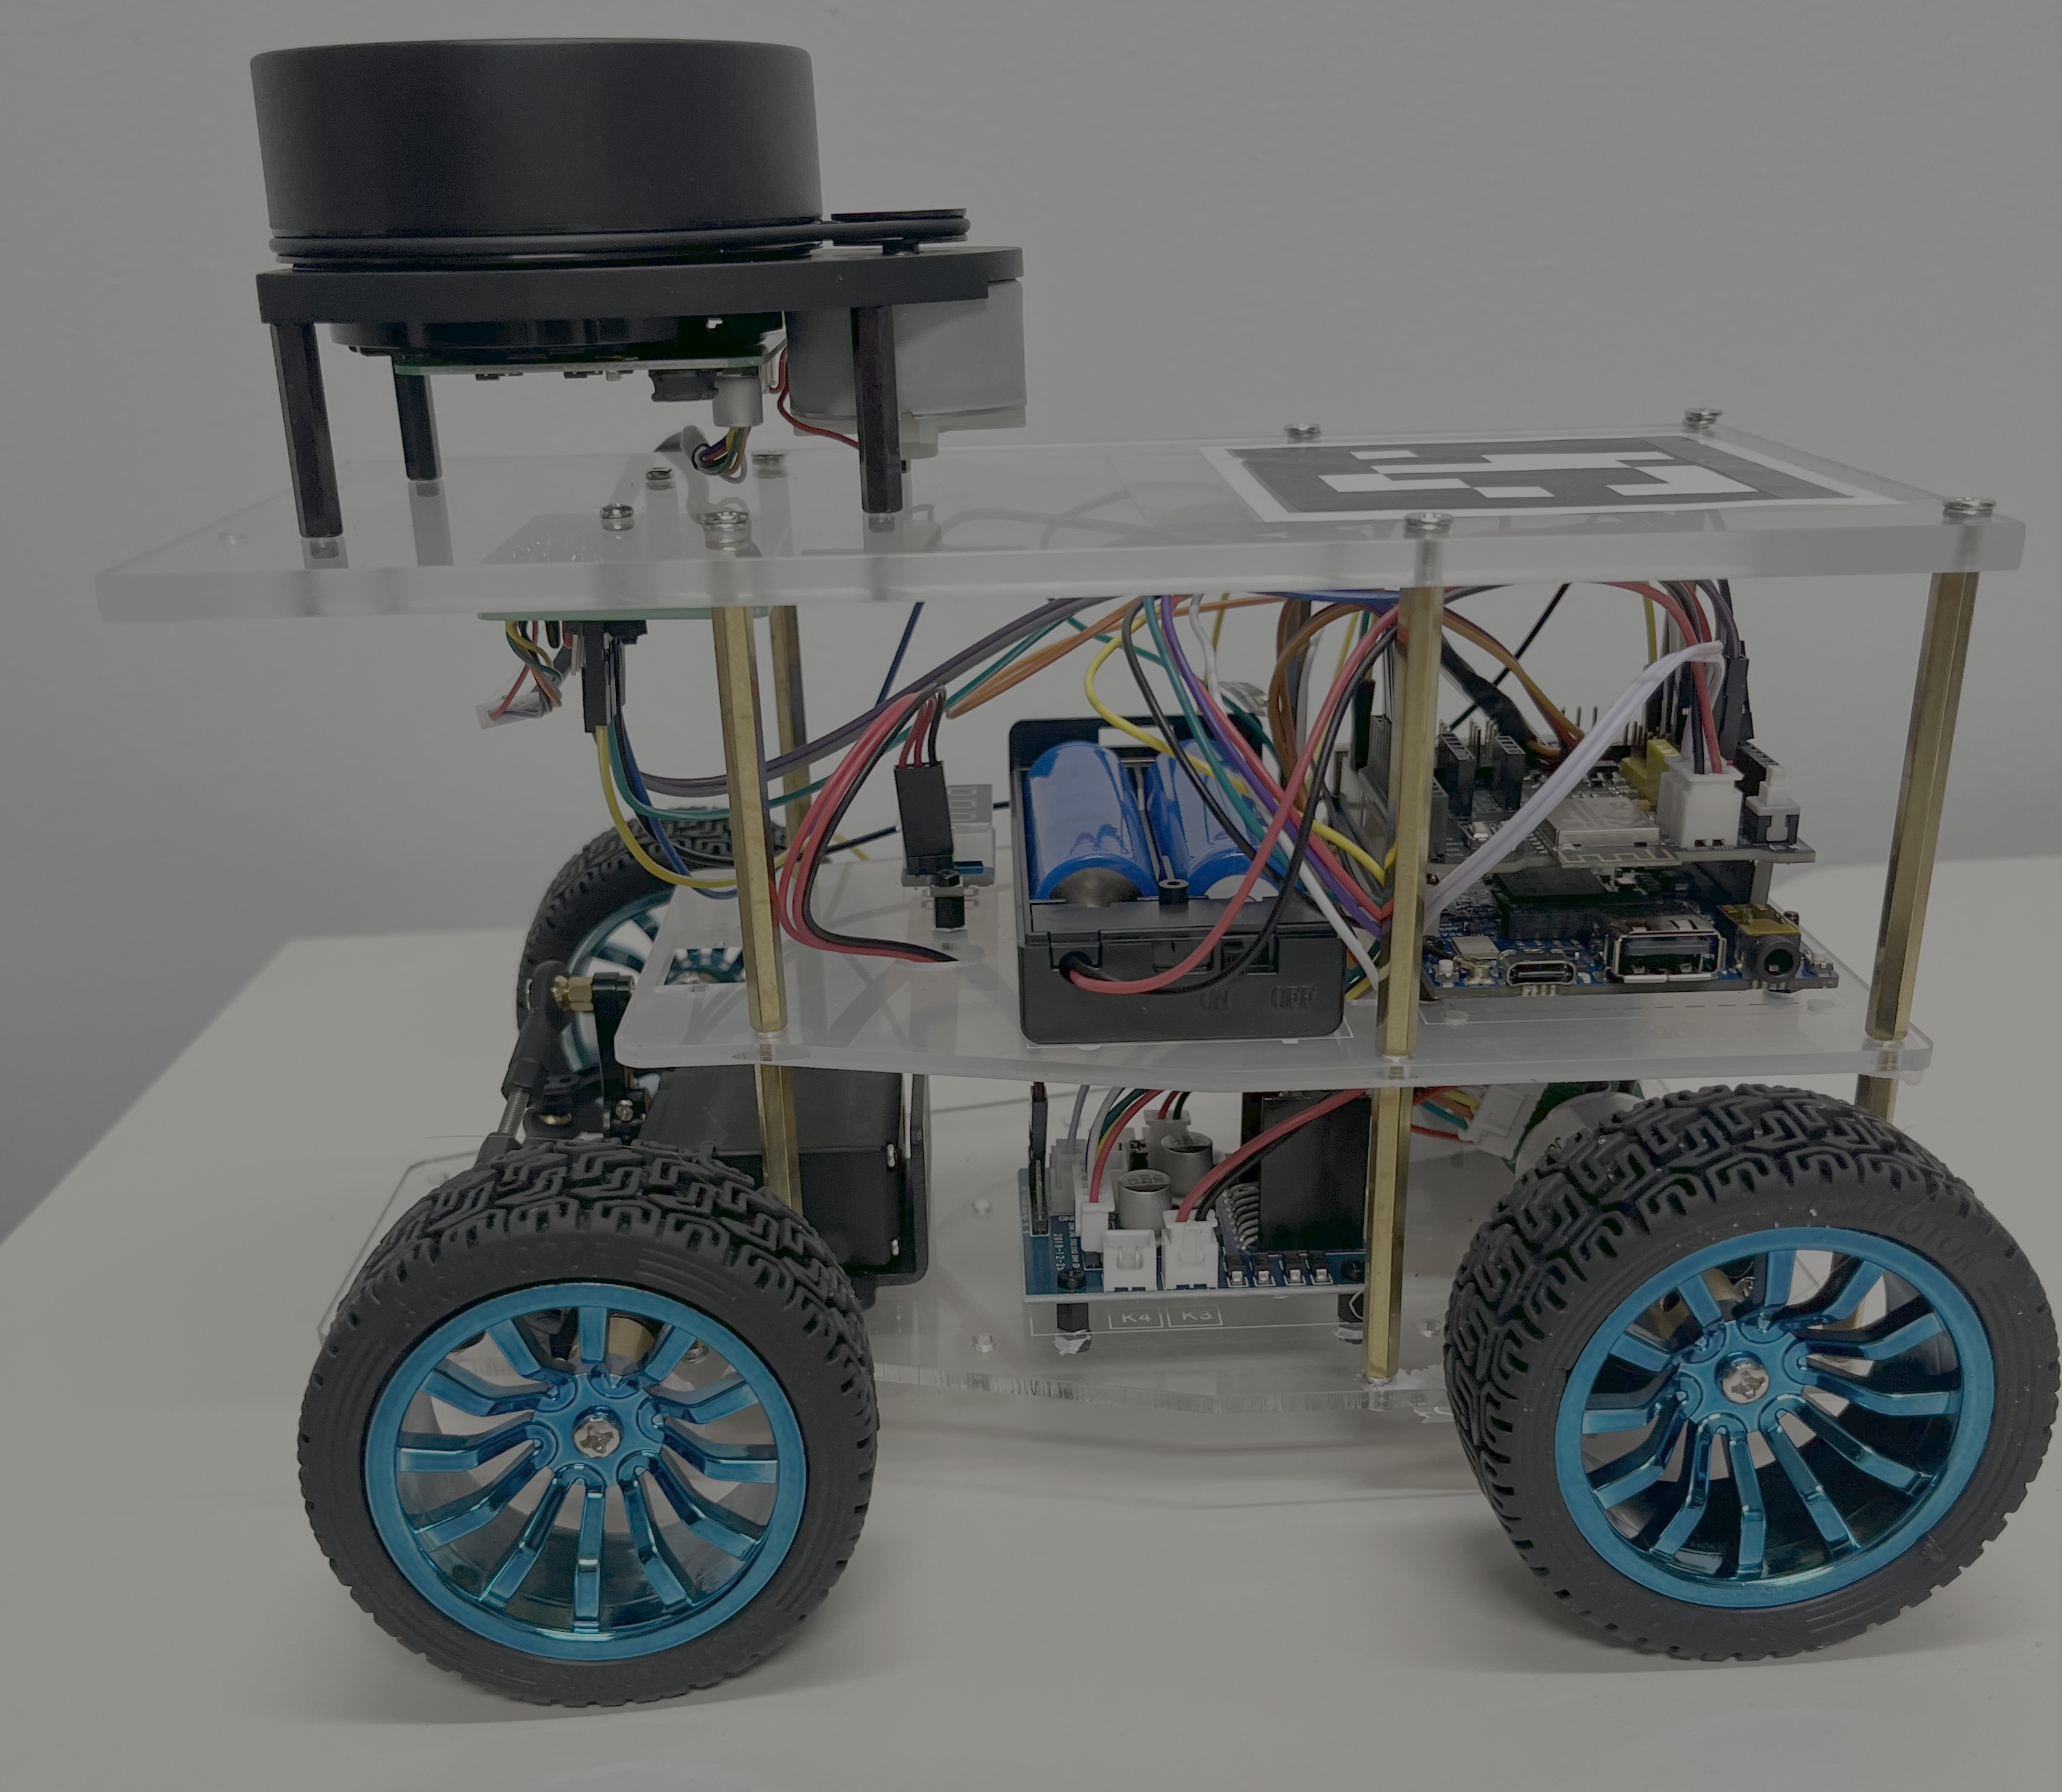
\includegraphics[width=0.42\textwidth]{a_robot_image.jpg}}
\caption{The four-wheeled robot platform with the RPLidar A1 mounted on the top deck.}
\label{fig:robot}
\end{figure}

\subsection{Euclidean Distance Transform Map}

The room boundary is represented as a closed polygon of wall segments. This polygon is rasterized onto a uniform grid of cell size $c{=}0.1$\,m. Interior cells are set to 1 (free) and wall/exterior cells to 0 (occupied).

The EDT is applied to this binary occupancy grid:
\begin{equation}
    d(i,j) = \min_{(i',j') \in \mathcal{W}} \left\lVert (i,j) - (i',j') \right\rVert_2 \cdot c
    \label{eq:edt}
\end{equation}
where $\mathcal{W}$ is the set of occupied cells. The scalar $d(i,j)$ encodes the straight-line clearance in metres to the nearest wall and is precomputed once via \texttt{scipy.ndimage.distance\_transform\_edt}. The surveyed room (${\approx}6.35\,\mathrm{m}\times5.25\,\mathrm{m}$) yields a $64\times53$ grid.

Figure~\ref{fig:edt} shows the resulting clearance field and the derived MPPI wall cost (described in Section~\ref{subsec:mppi}). The clearance field peaks at approximately 1.7\,m near the room centre and smoothly decays to zero at every wall boundary. The wall cost field shows the exponential barrier used by MPPI to repel trajectories from obstacles.

\begin{figure*}[htbp]
\centerline{
\includegraphics[width=\textwidth]{edt_heatmap.png}}
\caption{(a)~EDT clearance map: brighter colours indicate larger distance to the nearest wall. (b)~MPPI wall cost field with an example Dijkstra reference path (cyan) from a start (green) to a goal (red). The cost field is saturated at 80 for display; cells inside the wall boundary carry a hard penalty of 1000.}
\label{fig:edt}
\end{figure*}

\subsection{Dijkstra Reference Path}

A wall-clearance-penalized cost is assigned to each directed edge of the 8-connected grid graph:
\begin{equation}
    w_\mathrm{edge} = \frac{\ell_\mathrm{step}}{1 - e^{-d_\mathrm{min}/\alpha}}
    \label{eq:edge_weight}
\end{equation}
where $\ell_\mathrm{step}$ is the Euclidean step length ($c$ for cardinal, $c\sqrt{2}$ for diagonal), $d_\mathrm{min}$ is the minimum EDT clearance of the two endpoint cells, and $\alpha{=}5.0$\,m controls the decay sharpness. In open space ($d_\mathrm{min} \gg \alpha$) the denominator approaches 1 and the edge weight reduces to the Euclidean step; near walls ($d_\mathrm{min}\to 0$) the denominator collapses and the weight diverges, forcing paths to route away from obstacles.

The graph is pre-built as a sparse CSR matrix. When the operator sets a goal, a single call to \texttt{scipy.sparse.csgraph.dijkstra} from the robot's current PF mean position produces the globally optimal clearance-weighted reference path $\mathcal{P} = \{(x_k^p, y_k^p)\}_{k=1}^{P}$ in approximately 150--200\,ms. Because path planning runs only once per goal assignment, this cost does not affect real-time operation.

\subsection{Particle Filter Localization}
\label{subsec:pf}

A Monte Carlo Particle Filter~\cite{thrun} maintains $N{=}1{,}000$ weighted particles $\{(\mathbf{x}_t^{[i]}, w_t^{[i]})\}$ representing the posterior $p(\mathbf{x}_t \mid \mathbf{z}_{1:t}, \mathbf{u}_{1:t})$. Each particle is propagated via the robot's motion model using the encoder increment $\Delta e$ and steering angle $\alpha_t$; particles are then reweighted by a Gaussian likelihood over 50 LiDAR rays ray-cast against the map:
\begin{equation}
    w_t^{[i]} \propto \prod_{k} \exp\!\left(-\frac{(r_k - r_k^{[i]})^2}{2\sigma_r^2}\right), \quad \sigma_r^2 = 0.1\,\mathrm{m}^2
\label{eq:weight}
\end{equation}
Low-variance systematic resampling is applied every cycle. If the maximum weight falls below $10^{-9}$ for five consecutive cycles the particle set is reinitialized uniformly over free space. The PF mean $(\bar{x},\bar{y},\bar{\theta})$ is passed to MPPI as the current state.

\subsection{MPPI Control}
\label{subsec:mppi}

MPPI~\cite{williams} is a sampling-based receding-horizon controller. At each iteration it samples $K$ perturbed control sequences, rolls them forward through the motion model, scores them with a composite cost, and updates the nominal sequence via an importance-weighted average.

\subsubsection{Trajectory Sampling}
At each iteration $K{=}100$ steering sequences are sampled by perturbing the warm-started nominal:
\begin{equation}
    \tilde{u}_{k,t}^s = \mathrm{clip}(U_{t}^{s,\mathrm{nom}} + \epsilon_{k,t}),\; -20\degree,\; 20\degree), \quad \epsilon_{k,t} \sim \mathcal{N}(0,\,\sigma_\mathrm{steer}^2)
    \label{eq:u_sample}
\end{equation}
with $\sigma_\mathrm{steer}{=}10\degree$. The encoder component is held at the nominal rate $\bar{e}{=}85.5$ counts/step. All $K$ trajectories $\boldsymbol{\tau}_k \in \mathbb{R}^{(T+1)\times3}$ are integrated simultaneously using vectorized NumPy operations, with a single Python loop only over the $T{=}60$ time steps for the heading integration.

\subsubsection{Cost Function}
Each trajectory is scored by:
\begin{equation}
    \mathcal{C}_k = \mathcal{C}_k^\mathrm{wall} + \mathcal{C}_k^\mathrm{path} + \mathcal{C}_k^\mathrm{head} + \mathcal{C}_k^\mathrm{goal}
\label{eq:total_cost}
\end{equation}

\textit{Wall cost} — penalizes obstacle proximity via the EDT (see Fig.~\ref{fig:edt}b):
\begin{equation}
\mathcal{C}_k^\mathrm{wall} = \sum_{t=1}^{T} \begin{cases} 1000 & d(x_{k,t},y_{k,t}) \leq 0 \\ \lambda_w\, e^{-d(x_{k,t},y_{k,t})/0.5} & \text{otherwise} \end{cases}
\label{eq:wall_cost}
\end{equation}
with $\lambda_w{=}50$. The hard barrier of 1000 inside wall cells strongly discourages any trajectory that enters occupied space.

\textit{Path cost} — penalizes lateral deviation from $\mathcal{P}$:
\begin{equation}
    \mathcal{C}_k^\mathrm{path} = \lambda_p \sum_{t=1}^{T} \min_{j} \left\lVert (x_{k,t}, y_{k,t}) - (x_j^p, y_j^p) \right\rVert_2
\label{eq:path_cost}
\end{equation}
with $\lambda_p{=}1.0$.

\textit{Heading cost} — penalizes misalignment with the path tangent ($\lambda_h{=}1.5$).

\textit{Goal cost} — penalizes terminal distance to the goal:
\begin{equation}
    \mathcal{C}_k^\mathrm{goal} = \lambda_g \left\lVert (x_{k,T}, y_{k,T}) - \mathbf{x}^\mathrm{goal} \right\rVert_2, \quad \lambda_g{=}100
\label{eq:goal_cost}
\end{equation}

\subsubsection{Control Update and Stopping}
Trajectories are weighted by a softmax with temperature $\alpha{=}0.1$ and the nominal sequence updated as their weighted average, with the steering component clamped to $[\pm20\degree]$. The first element is transmitted; the sequence is shifted one step for warm-starting.

MPPI is deactivated when the PF mean reaches within $r_\mathrm{stop}{=}0.15$\,m of the goal, at which point a zero-velocity command is sent.

\section{Experiment Design}
\label{sec:design}

\subsection{Hardware Platform}
The robot is a four-wheeled Ackermann-steered vehicle built on an RC car chassis. An Arduino GIGA R1 drives a brushed DC motor (speed) and steering servo (angle). An RPLidar A1 is mounted on the top deck. An ESP32 module provides WiFi, exchanging 10-byte UDP datagrams with the laptop at 100\,ms intervals. The laptop runs a NiceGUI application with a 10\,Hz control-loop timer and a decoupled 2\,Hz map-visualization timer.

\subsection{Map Acquisition}
The room boundary was manually surveyed from LiDAR scans, producing 32 wall-segment endpoints forming a closed polygon of ${\approx}6.35\,\mathrm{m}\times5.25\,\mathrm{m}$.

\subsection{Particle Filter Validation}
Three initialization conditions were tested:
\begin{itemize}
    \item \textbf{Good Init:} particles seeded near the true pose.
    \item \textbf{Bad Init:} particles seeded ${\sim}1$\,m from truth.
    \item \textbf{Unknown Init:} particles uniformly distributed over all free cells.
\end{itemize}
Position spread $\sigma_{xy}$ and heading spread $\sigma_\theta$ were logged at 10\,Hz during a short driving circuit.

\subsection{MPPI Navigation Trial}
Once the PF converged ($\sigma_{xy}{<}0.3$\,m), a goal coordinate was set via the GUI, triggering Dijkstra path planning and activating MPPI. The robot navigated autonomously until the stop condition triggered. Per-stage timing was logged throughout.

\section{Experimental Results}
\label{sec:results}

\subsection{Particle Filter Convergence}

Figure~\ref{fig:convergence} shows particle spread versus time for all three initialization conditions. With a good initial pose the spread is near zero from the first scan. A bad initial pose causes a spike to ${\approx}230$\,cm at $t{\approx}0.5$\,s as the motion model propagates the erroneous estimate, before collapsing to below 5\,cm within ${\approx}1$\,s once LiDAR measurements correct the cloud. Unknown initialization begins at ${\approx}83$\,cm and also converges within ${\approx}1$\,s. Heading uncertainty $\sigma_\theta$ settles to $1\text{--}2\degree$ in all cases.

\begin{figure}[htbp]
\centerline{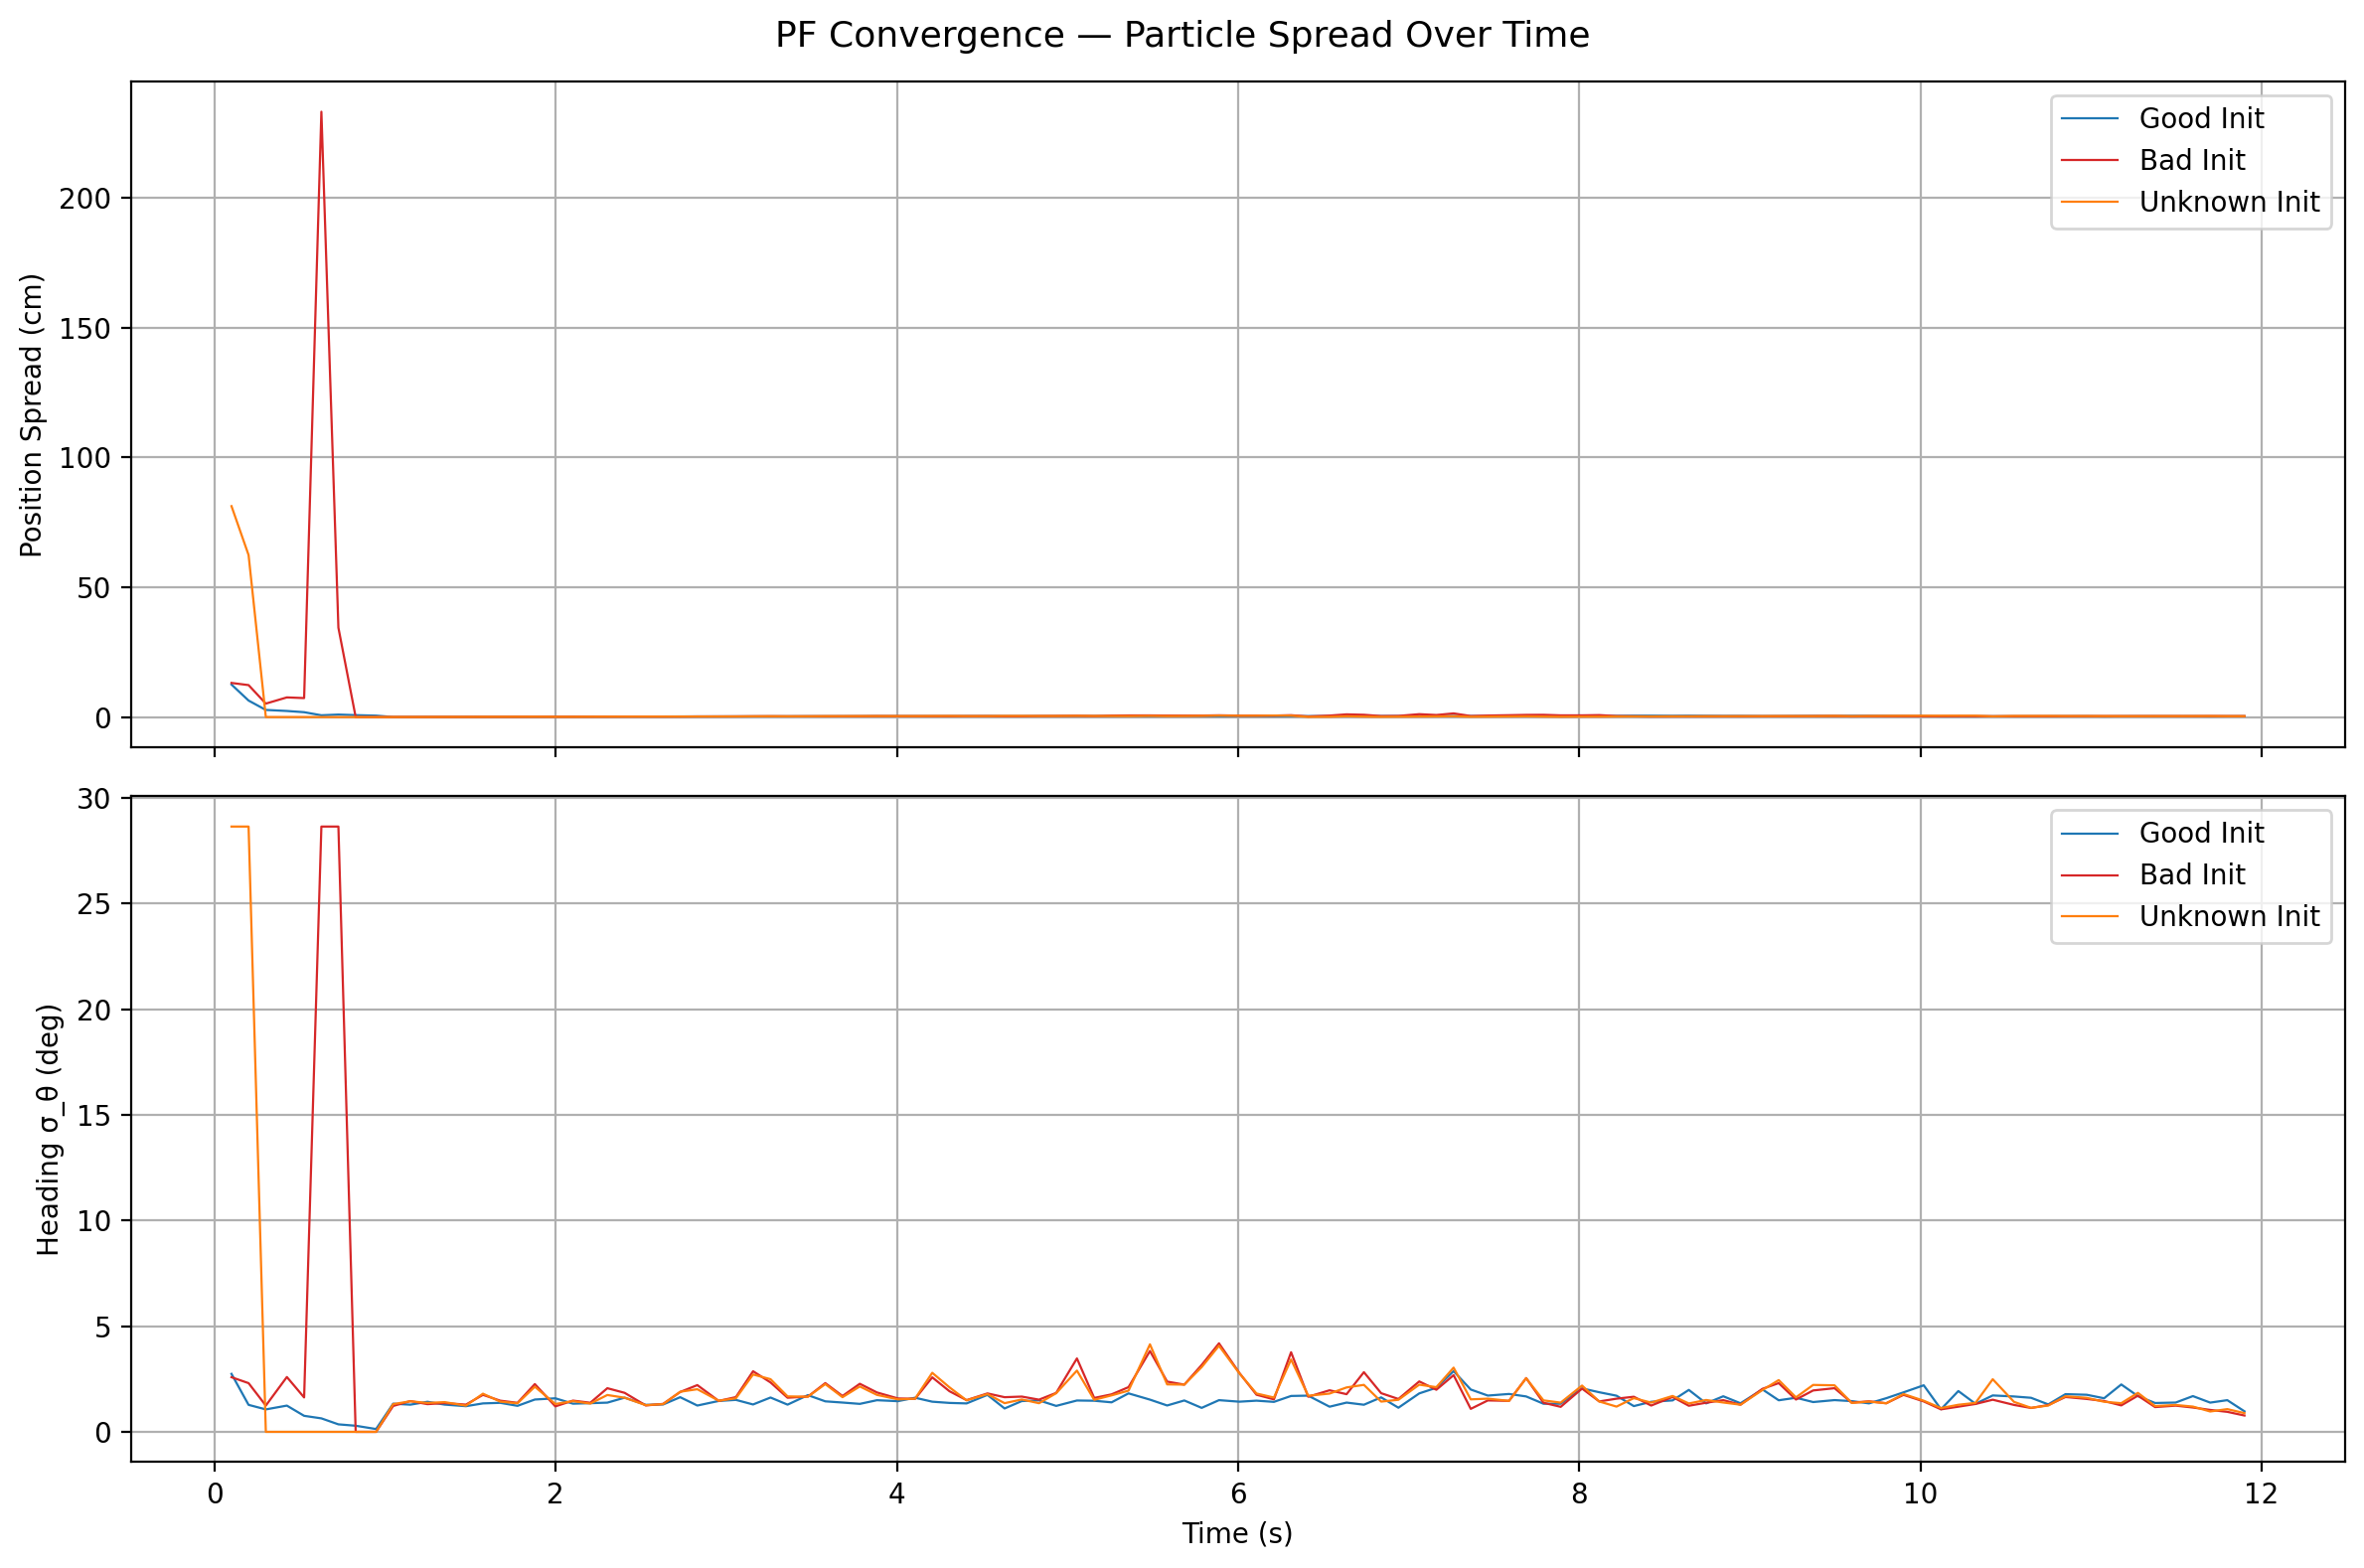
\includegraphics[width=0.48\textwidth]{convergence_plot.png}}
\caption{Particle spread for three initialization conditions. Position spread (top) and heading spread (bottom) both converge within 1\,s of robot motion.}
\label{fig:convergence}
\end{figure}

Figure~\ref{fig:trajectory} shows the PF mean trajectories with 95\% confidence ellipses. Ellipses collapse rapidly in the bad- and unknown-initialization cases, confirming fast convergence.

\begin{figure*}[htbp]
\centerline{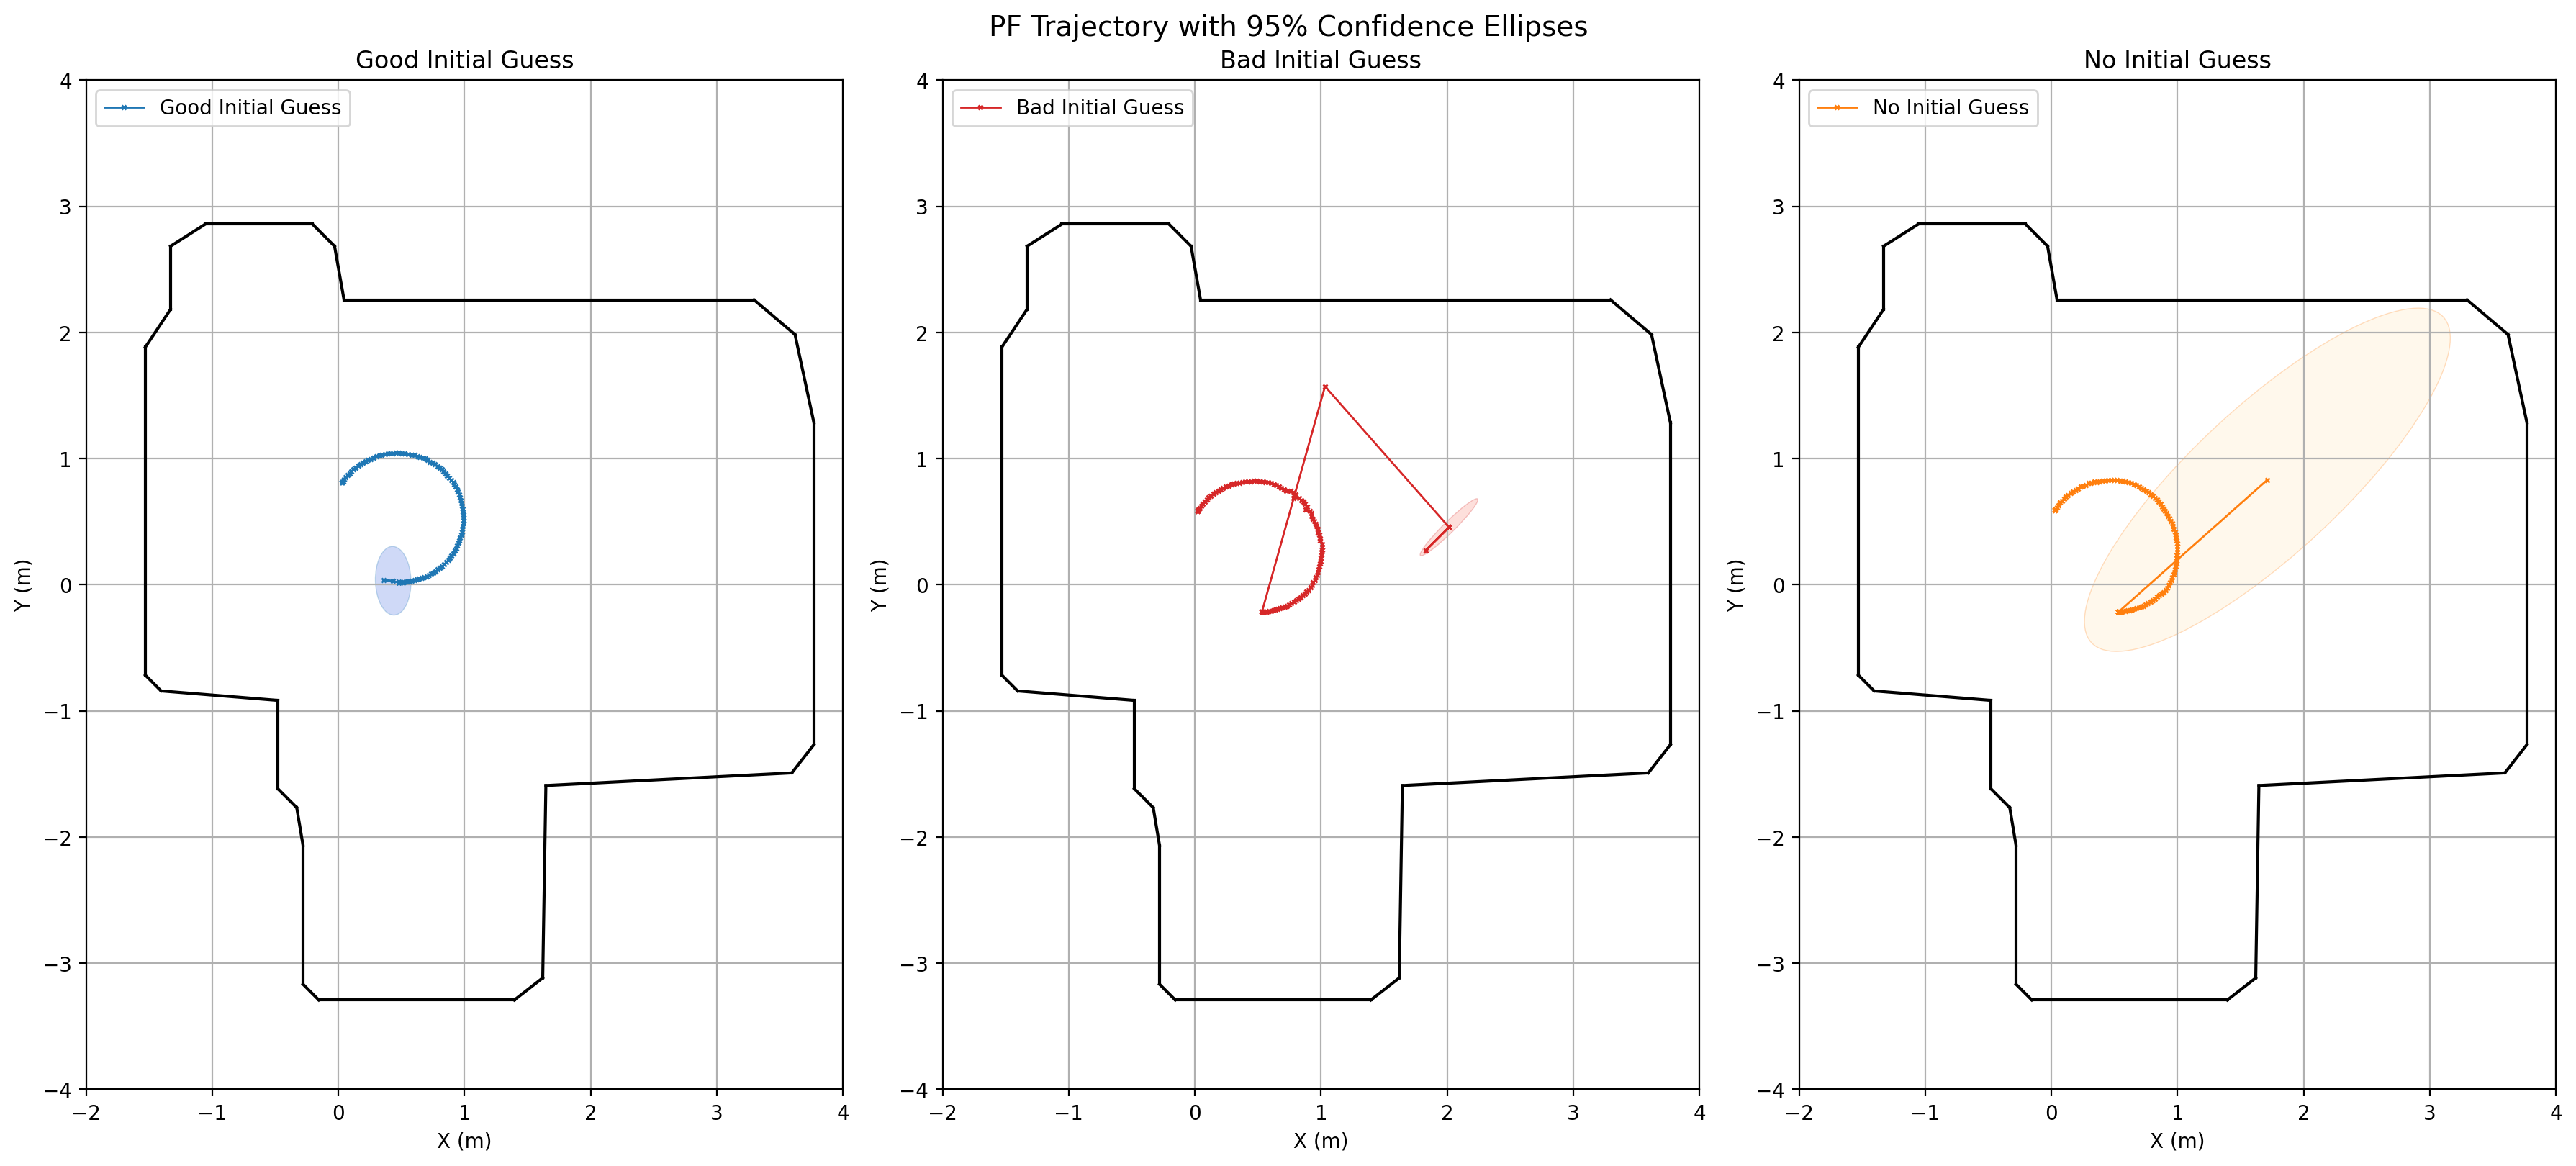
\includegraphics[width=\textwidth]{trajectory_plot.png}}
\caption{PF mean trajectories with 95\% confidence ellipses for good, bad, and unknown initial conditions. The black polygon is the room boundary.}
\label{fig:trajectory}
\end{figure*}

\subsection{Control Loop Timing}

Table~\ref{tab:timing} gives per-stage latencies during a full navigation run. The PF dominates at 38--40\,ms due to ray-casting 50 rays for 1\,000 particles. MPPI takes only 1.5--2.5\,ms because all $K{=}100$ trajectories are propagated simultaneously with vectorized NumPy operations, avoiding the $K \times T{=}6{,}000$ individual Python calls of a naive loop. Total loop latency of 40--42\,ms fits comfortably within the 100\,ms UDP cycle.

\begin{table}[htbp]
\centering
\caption{Per-stage control loop timing (50 LiDAR rays, $K{=}100$, $T{=}60$)}
\label{tab:timing}
\begin{tabular}{lcc}
\toprule
Stage & Mean (ms) & Max (ms) \\
\midrule
UDP Receive     & $<0.1$ & 0.1  \\
Particle Filter & 38.7   & 73.6 \\
MPPI            & 1.8    & 2.5  \\
UDP Send        & 0.1    & 0.1  \\
\midrule
\textbf{Total}  & \textbf{40.6} & \textbf{75.3} \\
\bottomrule
\end{tabular}
\end{table}

\subsection{MPPI Cost Tuning}

The wall cost parameters had the largest impact on navigation safety. An initial configuration of $\lambda_w{=}5$ with a 0.3\,m decay produced near-flat cost variation away from walls, causing the robot to clip corners. Increasing to $\lambda_w{=}50$ with a 0.5\,m decay created a steep barrier visible in Fig.~\ref{fig:edt}b, preventing sampled trajectories from approaching the wall boundary. The goal weight $\lambda_g$ was raised to 100 to overcome competition between path and heading costs near the goal. Table~\ref{tab:mppi_params} lists the final parameters.

\begin{table}[htbp]
\centering
\caption{Final MPPI hyperparameters}
\label{tab:mppi_params}
\begin{tabular}{lll}
\toprule
Parameter & Symbol & Value \\
\midrule
Trajectories       & $K$                     & 100 \\
Horizon            & $T$                     & 60 steps \\
Step time          & $\Delta t$              & 0.1\,s \\
Temperature        & $\alpha$                & 0.1 \\
Steering noise     & $\sigma_\mathrm{steer}$ & $10\degree$ \\
Wall weight        & $\lambda_w$             & 50 \\
Wall decay radius  & ---                     & 0.5\,m \\
Path weight        & $\lambda_p$             & 1.0 \\
Heading weight     & $\lambda_h$             & 1.5 \\
Goal weight        & $\lambda_g$             & 100 \\
Goal-stop radius   & $r_\mathrm{stop}$       & 0.15\,m \\
\bottomrule
\end{tabular}
\end{table}

\section{Conclusion}
\label{sec:conclusion}

A complete autonomous navigation pipeline was implemented and validated on a four-wheeled robot. The EDT map provides a compact, globally consistent representation of wall clearance that simultaneously drives Dijkstra path planning and the MPPI obstacle-avoidance cost. The Particle Filter converged from arbitrary initial positions within ${\approx}1$\,s of motion with final heading uncertainty below $2\degree$. The vectorized MPPI implementation completed each iteration in under 2.5\,ms, leaving the 100\,ms control budget dominated by PF ray-casting at 38--40\,ms.

Key tuning insight: the wall cost decay radius is the most influential MPPI parameter. A radius below ${\approx}0.5$\,m produces nearly flat cost across the navigable area, making the controller indifferent to wall proximity. Future work could replace the static Dijkstra reference with online replanning when the LiDAR detects transient obstacles, and reduce PF cost by porting the ray-caster to a compiled NumPy/Cython extension.

\begin{thebibliography}{00}
\bibitem{thrun} S.~Thrun, W.~Burgard, and D.~Fox, \textit{Probabilistic Robotics}. Cambridge, MA: MIT Press, 2005.
\bibitem{williams} G.~Williams, P.~Drews, B.~Goldfain, J.~M.~Rehg, and E.~A.~Theodorou, ``Aggressive driving with model predictive path integral control,'' in \textit{Proc. IEEE ICRA}, Stockholm, Sweden, 2016, pp.~1433--1440.
\bibitem{meijster} A.~Meijster, J.~B.~T.~M.~Roerdink, and W.~H.~Hesselink, ``A general algorithm for computing distance transforms in linear time,'' in \textit{Mathematical Morphology and its Applications to Image and Signal Processing}, Springer, 2000, pp.~331--340.
\bibitem{dijkstra} E.~W.~Dijkstra, ``A note on two problems in connexion with graphs,'' \textit{Numerische Mathematik}, vol.~1, pp.~269--271, 1959.
\bibitem{lecture_notes} C.~Clark, ``Lab 05 --- Autonomous Navigation,'' ROB-GY 6213 Robot Localization and Navigation, New York University, 2026.
\bibitem{imaginelenses} Imaginelenses, ``NYU\_ROB\_GY\_6213,'' GitHub, [Online]. \texttt{https://github.com/imaginelenses/NYU\_ROB\_GY\_6213}
\end{thebibliography}

\end{document}
